%!TEX root=../GaugeCNNTheory.tex


\subsection{تناوب‌پذیری ایزومتری}
\label{sec:gauge_conv_isom_equiv}


\begin{SCfigure}
	\centering
	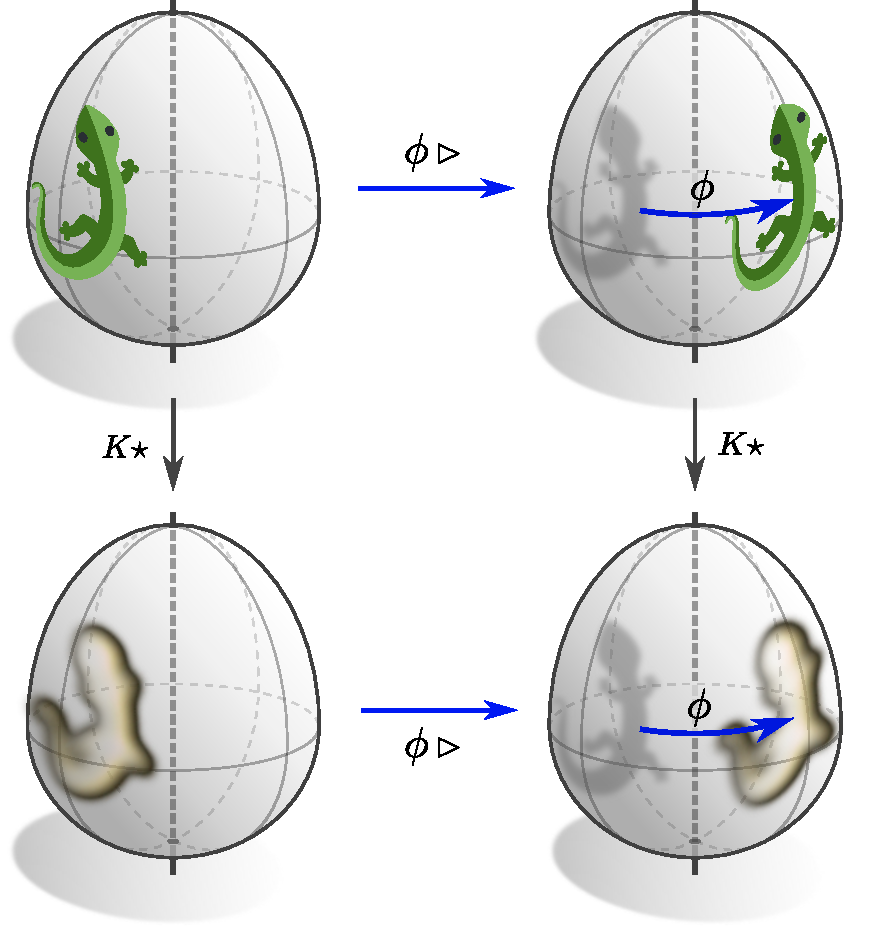
\includegraphics[width=.56\textwidth]{figures/lizard_conv_egg.pdf}
	\captionsetup{width=.89\textwidth}
	\caption[]{\small
		گفته می‌شود یک لایه شبکه تحت ایزومتری‌ها تناوب‌پذیر است زمانی که با عمل آن‌ها بر میدان‌های ویژگی جابجا می‌شود.
		$\GM$-کانولوشن‌ها طراحی شده‌اند تا نسبت به آن ایزومتری‌هایی $\phi\in \IsomGM$ که تقارن‌های $G$-ساختار هستند، تناوب‌پذیر باشند.
		در معادلات، کانولوشن $K\star$ تحت عمل ایزومتری $\phi$ تناوب‌پذیر است زمانی که رابطه
		$K \star \big( \phi\rhd\! \fin \big) = \phi\rhd\! \big(K \star \fin \big)$
		را برای هر انتخابی از میدان ورودی~$\fin$ برآورده کند.
		این رابطه توسط نمودار جابجایی در معادله~\eqref{cd:isometry_equivariance_conv_mapsto} بصری‌سازی شده است که تفسیر گرافیکی آن در این شکل نشان داده شده است.
		\\[1ex]
		اینکه $\GM$-کانولوشن‌ها $\IsomGM$-تناوب‌پذیر هستند بر این حقایق تکیه دارد که
		۱) کرنل‌ها در کل منیفولد به اشتراک گذاشته می‌شوند،
		۲) ایزومتری‌ها عقب‌کشی انتقال‌دهنده میدان‌های ویژگی را حفظ می‌کنند و
		۳) اینکه $\IsomGM$ تبدیل‌های گیج با مقدار $G$ را القا می‌کند که توسط $G$-استیریبل بودن کرنل در نظر گرفته می‌شود.
		{\\
			\color{gray}
			\scriptsize
			(مارمولک‌ها تحت مجوز \lr{Creative Commons Attribution 4.0 International}
			\href{https://github.com/twitter/twemoji/blob/gh-pages/LICENSE-GRAPHICS}{\underline{اقتباس شده}}
			با مجوز \lr{Twitter}.)
		}
		\\[0ex]
	}
	\label{fig:lizard_conv_egg}
\end{SCfigure}


با توجه به اینکه یک منیفولد تقارن‌هایی نشان می‌دهد، معمولاً مطلوب است که شبکه‌های عصبی این تقارن‌ها را رعایت کنند، یعنی تحت عمل آن‌ها بر میدان‌های ویژگی تناوب‌پذیر باشند.
$\GM$-کانولوشن‌ها طراحی شده‌اند تا $\IsomGM$-تناوب‌پذیر باشند، که به این معنی است که آن‌ها با عمل ایزومتری‌ها در $\IsomGM$ بر میدان‌های ویژگی جابجا می‌شوند، همانطور که در شکل~\ref{fig:lizard_conv_egg} بصری‌سازی شده است.%
\footnote{
	به یاد داشته باشید که عمل بر میدان‌های ویژگی مستقل از مختصات $\GM$ تنها برای ایزومتری‌های حفظ‌کننده $G$-ساختار در $\IsomGM$ قابل تعریف است.
	بنابراین حتی امکان تعریف مفهوم تناوب‌پذیری ایزومتری برای ایزومتری‌هایی که تقارن‌های $G$-ساختار نیستند وجود ندارد.
	توجه داشته باشید که این بدون از دست دادن کلیت است زیرا همیشه می‌توان گروه ساختار $G=\O{d}$ را انتخاب کرد که برای آن $\IsomGM=\IsomM$ با کل گروه ایزومتری منطبق می‌شود.
}.
در معادلات، $\GM$-کانولوشن $K\star$ تناوب‌پذیر است زمانی که رابطه
\begin{align}\label{eq:isometry_equivariance_conv_def_33}
	K \star \big( \phi\rhd\! \fin \big) \ =\ \phi\rhd\! \big( K \star \fin \big)
	\qquad \forall\ \ \phi\in \IsomGM
\end{align}
را برای هر میدان ورودی ممکن $\fin$ برآورده کند، یعنی زمانی که نمودار زیر جابجا باشد:

\begin{equation}\label{cd:isometry_equivariance_conv_mapsto}
	\begin{tikzcd}[column sep=60pt, row sep=35, font=\normalsize]
		\fin
		\arrow[r, "\phi\,\rhd", mapsto]
		\arrow[d, "K\star"', mapsto]
		&
		\phi\,\rhd \fin
		\arrow[d, "K\star", mapsto]
		\\
		\fout
		\arrow[r, "\phi\,\rhd"', mapsto]
		&
		\phi\,\rhd \fout
	\end{tikzcd}
\end{equation}


به عنوان اولین قدم به سوی اثبات تناوب‌پذیری ایزومتری $\GM$-کانولوشن‌ها، به یاد بیاورید که آن‌ها به صورت نقطه‌ای به عنوان انقباض یک کرنل $K$ با عقب‌کشی انتقال‌دهنده $[\Expspfin]^A$ از میدان ورودی~$\fin$ تعریف می‌شوند.
از آنجا که ایزومتری‌ها به طور تعریف هندسه ریمانی~$M$ را حفظ می‌کنند، به ویژه نگاشت نمایی ریمانی و انتقال‌دهنده‌های لوی-چیویتا را حفظ می‌کنند؛ به بخش~\ref{sec:isom_expmap_transport} و شکل~\ref{fig:isom_exp_transport} مراجعه کنید.%
\footnote{
	به طور کلی‌تر، هر زمان که یک اتصال جایگزین $G$-سازگار برای انتقال بردارهای ویژگی انتخاب شود، فرض می‌کنیم این اتصال تحت عمل $\IsomGM$ ناوردا باشد؛ به بخش~\ref{sec:isom_expmap_transport} مراجعه کنید.
	این فرض برای همه مدل‌هایی که در بررسی ادبیات در بخش~\ref{part:literature_review} پوشش داده شده‌اند، برآورده می‌شود.
}
این امر دلالت دارد بر اینکه عقب‌کشی انتقال‌دهنده میدان پیش‌برده $\phi\rhd\fin$ در $\phi(p)$ تنها با تبدیل گیج القا شده توسط ایزومتری از عقب‌کشی انتقال‌دهنده میدان اصلی $\fin$ در $p$ متفاوت خواهد بود، یعنی:

\begin{align}\label{eq:transporter_pullback_pushforward_field}
	\big[\mkern-2mu \Expsphip (\phi\rhd\fin) \big]^A\ =\ 
	\rhoin\big( g_\phi^{A\widetilde{A}}(p)\big) \circ \big[\mkern-2mu \Expspfin\big]^{\widetilde{A}} \circ g_\phi^{A\widetilde{A}}(p)^{-1} \,;
\end{align}
مقایسه کنید با معادله~\eqref{eq:trafo_law_transporter_pullback} و، برای فرمول‌بندی مستقل از مختصات، قضیه~\ref{thm:transporter_pullback_isometry_action}.

با توجه به این همانی، تناوب‌پذیری ایزومتری $\GM$-کانولوشن‌ها
توسط محاسبه ساده زیر اثبات می‌شود که به طور اساسی از $G$-استیریبل بودن کرنل قالب~$K$ برای توضیح عمل گیج القا شده توسط ایزومتری استفاده می‌کند:

\begin{align}
	\big[ K \star (\phi \rhd \fin) \big]^A (\phi(p))
	\ \overset{(1)}{=}&\ \ 
	\int_{\R^d} K(\mathscr{v})\  \big[\mkern-2mu \Expsphip (\phi\rhd\fin) \big]^A (\mathscr{v})\ d\mathscr{v} \notag \\
	\ \overset{(2)}{=}&\ \ 
	\int_{\R^d} K(\mathscr{v})\ 
	\Big[ \rhoin\pig( g_\phi^{A\widetilde{A}}(p)\pig) \big[\mkern-2mu \Expspfin\big]^{\widetilde{A}} \pig(g_\phi^{A\widetilde{A}}(p)^{-1} \mathscr{v} \pig) \Big]\ d\mathscr{v} \notag \\
	\ \overset{(3)}{=}&\ \ 
	\int_{\R^d} \Big[ K\pig( g_\phi^{A\widetilde{A}}(p)\, \tilde{\mathscr{v}}\pig)\ \rhoin\pig( g_\phi^{A\widetilde{A}}(p)\pig) \Big]\ 
	\big[\mkern-2mu \Expspfin\big]^{\widetilde{A}} (\tilde{\mathscr{v}})\ 
	\pig|\mkern-3mu\det g_\phi^{A\widetilde{A}}(p)\pig|\; d\tilde{\mathscr{v}} \notag \\
	\ \overset{(4)}{=}&\ \ 
	\int_{\R^d} \Big[\rhoout\pig( g_\phi^{A\widetilde{A}}(p)\pig)  K\big(\tilde{\mathscr{v}}\big) \Big]\ 
	\big[\mkern-2mu \Expspfin\big]^{\widetilde{A}} (\tilde{\mathscr{v}})\ d\tilde{\mathscr{v}} \notag \\
	\ \overset{(5)}{=}&\ \ 
	\rhoout\big( g_\phi^{A\widetilde{A}}(p) \big) \cdot \fout^{\widetilde{A}}(p) \notag \\
	\ \overset{(6)}{=}&\ \ 
	\big[ \phi \rhd \fout \big]^A (\phi(p)) \notag \\
	\ \overset{(7)}{=}&\ \ 
	\big[ \phi \rhd \big(K \star \fin\big) \big]^A (\phi(p))
\end{align}
قدم اول از تعریف $\GM$-کانولوشن‌ها در معادله~\eqref{eq:gauge_conv_coord_expression} پیروی می‌کند در حالی که قدم دوم تبدیل گیج القا شده را طبق معادله~\eqref{eq:transporter_pullback_pushforward_field} وارد کرد.
جایگزینی از $\mathscr{v}$ به $\tilde{\mathscr{v}} = g_\phi^{A\widetilde{A}}(p)^{-1} \mkern1mu \mathscr{v}$ قدم سوم را توجیه می‌کند.
در قدم چهارم $G$-استیریبل بودن کرنل قالب، یعنی معادله~\eqref{eq:kernel_constraint}، اعمال می‌شود (معادله~\eqref{eq:IsomGM_coord_in_G_24} را به یاد بیاورید که بیان می‌کند تبدیل‌های گیج القا شده توسط $\IsomGM$ دارای مقدار $G$ هستند).
نتیجه این است که بردار ویژگی خروجی حاصل توسط تبدیل گیج القا شده تبدیل می‌شود.
پس از شناسایی این امر به عنوان بیان مختصاتی پیش‌برد میدان خروجی در معادله~\eqref{eq:feature_field_trafo_in_coords}، گزاره پیروی می‌کند.
از آنجا که همه قدم‌ها برای ایزومتری‌های دلخواه در $\IsomGM$ معتبر هستند، می‌بینیم که \emph{$\GM$-کانولوشن‌ها به طور خودکار نسبت به هر ایزومتری حفظ‌کننده $G$-ساختار تناوب‌پذیر هستند}.
آن‌ها لزوماً نسبت به ایزومتری‌های عمومی در $\IsomM$ که ممکن است $G$-ساختار را رعایت نکنند تناوب‌پذیر \emph{نیستند}، با این حال، تناوب‌پذیری کامل ایزومتری برای گروه‌های ساختار متعامد $G=\O{d}$ (یا ابرگروه‌های آن) تضمین شده است.



\paragraph{میدان‌های کرنل ناوردا:}
تحلیل عمیق‌تری از تناوب‌پذیری ایزومتری تبدیل‌های میدان کرنل عمومی را می‌توان در بخش‌های~\ref{sec:isometry_equivariance} و~\ref{sec:quotient_kernel_fields} یافت.
نتیجه اصلی این بررسی قضیه~\ref{thm:isometry_equivariant_kernel_field_trafos} است که بیان می‌کند \emph{تناوب‌پذیری ایزومتری یک تبدیل میدان کرنل، ناوردایی ایزومتری میدان کرنل آن را نتیجه می‌دهد و بالعکس}.
شکل~\ref{fig:isom_invariant_kernel_field_multiple_orbits} چنین میدان کرنل ناوردایی را بصری‌سازی می‌کند که ملزم به اشتراک وزن‌ها بر روی مدارات عمل ایزومتری است.
ناوردایی مورد نیاز میدان کرنل از نظر شهودی قابل فهم است زیرا تناوب‌پذیری ایزومتری مطمئناً نیازمند ثابت بودن استنتاج شبکه بر روی هر مدار است.
این نتیجه انتزاعی تناوب‌پذیری ایزومتری $\GM$-کانولوشن‌ها را با مشاهده اینکه میدان‌های کرنل $\GM$-کانولوشنی -- که توسط یک کرنل قالب منفرد و مشترک تعیین می‌شوند -- تحت ایزومتری‌ها در $\IsomGM$ ناوردا هستند، نتیجه می‌دهد؛ به قضیه~\ref{thm:isom_equiv_GM_conv} و شکل~\ref{fig:intro_invariant_kernel_fields_plane} مراجعه کنید.
$G$-استیریبل بودن کرنل قالب بدین ترتیب ناوردایی کرنل‌ها تحت عمل زیرگروه‌های پایدار کننده گروه ایزومتری را توضیح می‌دهد.



\paragraph{فضاهای همگن:}
در حالی که تقاضای تناوب‌پذیری ایزومتری نیازمند آن است که کرنل‌ها بر روی مدارات گروه ایزومتری به اشتراک گذاشته شوند، به طور کلی نیازمند اشتراک وزن کانولوشنی در کل منیفولد نیست.
یک استثنای مهم حالت منیفلدهایی است که \emph{فضاهای همگن} گروه ایزومتری خود هستند، مانند $\R^d$ یا کره $S^2$.
به طور تعریف، عمل ایزومتری در چنین فضاهایی متعدی است، یعنی تنها یک مدار منفرد وجود دارد.
در نتیجه، تنها یک کرنل مستقل وجود خواهد داشت که از طریق عمل گروه ایزومتری در کل فضا به اشتراک گذاشته می‌شود.
قضیه~\ref{thm:GM_conv_homogeneous_equivalence} در بخش~\ref{sec:quotient_kernel_fields} ثابت می‌کند که \emph{تبدیل‌های میدان کرنل تناوب‌پذیر ایزومتری در فضاهای همگن لزوماً کانولوشن‌های مستقل از مختصات هستند}.
این مشاهده پیوند رسمی بین نظریه ما و کارهای قبلی در مورد شبکه‌های کانولوشنی در فضاهای همگن
توسط~\citet{Kondor2018-GENERAL}، \citet{Cohen2019-generaltheory} و~\citet{bekkers2020bspline} برقرار می‌کند
که کانولوشن‌ها را از طریق تناوب‌پذیری آن‌ها نسبت به تقارن‌های سراسری فضای زیرین تعریف می‌کنند.






\paragraph{تناوب‌پذیری دیفئومورفیسم:}
خواننده ممکن است تعجب کند که آیا امکان کاملاً دیفئومورفیسم تناوب‌پذیر کردن CNNهای مستقل از مختصات ما وجود دارد یا نه.
همانطور که به راحتی می‌توان دید، عملیات نقطه‌ای از بخش~\ref{sec:pointwise_operations}، یعنی $\onexones$، بایاس‌ها و غیرخطی‌ها، از قبل دیفئومورفیسم تناوب‌پذیر هستند.
به طور خاص، بگذارید

\begin{align}\label{eq:DiffGM_def_part1}
	\DiffGM\ :=\ \pig\{ \phi \in \Diff(M) \ \pig|\ 
	\big[\phi_*(e_i)\big]_{i=1}^d \in \GM \quad \forall\ [e_i]_{i=1}^d \in \GM \pig\} \,\ \leq\ \Diff(M)
\end{align}
زیرگروه دیفئومورفیسم‌های حفظ‌کننده $G$-ساختار باشد، یعنی آنالوگ معادله~\eqref{eq:IsomGM_def_24} بدون نیاز به اینکه~$\phi$ ایزومتری باشد.
مشابه معادله~\eqref{eq:IsomGM_coord_in_G_24} و قضیه~\ref{thm:isom_GM_in_coords}، بیان‌های مختصاتی (تبدیل‌های گیج القا شده) دیفئومورفیسم‌های حفظ‌کننده $G$-ساختار تضمین شده‌اند که مقادیری در $G$ بگیرند، یعنی:
\begin{align}
	\phi \in \DiffGM \quad \Longleftrightarrow \quad g_\phi^{A\widetilde{A}}(p) \in G\ \ \ \forall\ p \mkern-1mu\in\mkern-2mu M \,.
\end{align}
$G$-تناوب‌پذیری توابع قالب نقطه‌ای مشترک تضمین خواهد کرد که آن‌ها با این تبدیل‌های گیج القا شده توسط $\DiffGM$ جابجا شوند -- و بنابراین با خود عمل دیفئومورفیسم فعال.


از طرف دیگر، $\GM$-کانولوشن‌ها با کرنل‌های گسترده فضایی، به طور کلی نسبت به دیفئومورفیسم‌ها تناوب‌پذیر \emph{نیستند}.
دلیل این امر آن است که عقب‌کشی انتقال‌دهنده $\Expspf$ بر نگاشت‌های نمایی تکیه می‌کند که ذاتاً ساختارهای ریمانی هستند که با دیفئومورفیسم‌ها جابجا نمی‌شوند.
با این حال، از آنجا که کرنل‌ها $G$-استیریبل هستند، تناوب‌پذیری $\DiffGM$ باید در حد صفر رفتن پشتیبانی کرنل همچنان برقرار باشد.
با توجه به اینکه کرنل‌های کانولوشن در کاربردهای معمول یادگیری عمیق کاملاً کوچک هستند، تناوب‌پذیری دیفئومورفیسم باید در عمل تقریباً برقرار باشد.



\paragraph{تناوب‌پذیری آفین:}
فضاهای اقلیدسی حالت خاصی را تشکیل می‌دهają زیرا امکان $\GM$-کانولوشن‌هایی را فراهم می‌کنند که تحت عمل \emph{گروه‌های آفین}~$\Aff(G)$ تناوب‌پذیر هستند.
اینکه چنین است به این حقیقت تکیه دارد که نگاشت نمایی در فضاهای اقلیدسی نه تنها با عمل ایزومتری‌ها بلکه به طور کلی‌تر با تبدیل‌های آفین جابجا می‌شود.
تناوب‌پذیری گروه آفین $\GM$-کانولوشن‌های اقلیدسی در بخش~\ref{sec:euclidean_affine_equiv} اثبات شده است.